\lab{Algorithms}{Numerical Derivatives}{Numerical Derivatives}
\label{Ch:Numerical Derivatives}

\objective{Understand and implement finite difference approximations of the derivative. This lab focuses on functions from $\mathbb{R} \to \mathbb{R}$, while a later lab focuses on the multidimensional case.}

The derivative of a function at a point is formally defined as

\begin{equation}
\label{eqn:deriv}
f'(x) = \lim_{h\rightarrow 0} \frac{f(x + h)-f(x)}{h}.
\end{equation}

In most real world applications we will be solving problems using computers. How does a computer calculate a limit? In short it can't. Computers can only approximate functions at specific points, and the notion of a limit graces infinity in a way that a computer never can.

So how can we use a computer to find the derivative of a function, particularly when we can't differentiate the function by hand? We use methods known as finite difference methods. For example suppose that in equation \ref{eqn:deriv}, instead of taking a limit we just pick a particularly small value for h. Then we have

\begin{equation*}
f'(x) \approx \frac{f(x + h)-f(x)}{h}
\end{equation*}

This is known as the first order forward difference approximation of the derivative.

How do we know the quality of this approximation? We can use Taylor's formula to find

\begin{equation*}
f(x_0 + h) = f(x_0) + hf'(x_0) + h^2/2 f''(\xi),\hspace{5mm} \xi \in (x_0,x_0 + h)
\end{equation*}

Which can be also expressed as

\begin{equation*}
f'(x_0) = \frac{f(x_0 + h) - f(x)}{h} + \frac{h}{2}f''(\xi) = \frac{f(x_0 + h) - f(x)}{h} + O(h)
\end{equation*}

Here we use the big-O notation to denote that the errors are bounded by some constant multiplied by $h$.

We can use Taylor expansions to find approximations that have different big-O error bounds, up to any polynomial of arbitrary degree. Tables \ref{Table:CDiff} and \ref{Table:FDiff} offer the coefficients for centered and forward difference schemes.

\begin{table}
\begin{center}
\begin{tabular}{|c|c|c|c|c|c|c|c|c|}
\hline
Derivative & Accuracy & -3 & -2 & -1 & 0 & 1 & 2 & 3 \\ \hline
 & 2 & & & -1/2 & 0 & 1/2 & & \\ \cline{2-9}
 1 & 4 & & 1/12 & -2/3 &  0 & 2/3 & -1/12 & \\ \cline{2-9}
  & 6 & -1/60 & 3/20 & -3/4 & 0 & 3/4 & -3/20 & 1/60 \\ \hline
  & 2 & & & 1 & -2 & 1 & & \\ \cline{2-9}
 2 & 4 & & -1/12 & 4/3 &  -5/2 & 4/3 & -1/12 & \\ \cline{2-9}
  & 6 & 1/90 & -3/20 & 3/2 & -49/18 & 3/2 & -3/20 & 1/90 \\ \hline
\end{tabular}
\caption{Centered Difference Coefficients}
\label{Table:CDiff}
\end{center}
\end{table}

\begin{table}
\begin{center}
\begin{tabular}{|c|c|c|c|c|c|c|}
\hline
Derivative & Accuracy & 0 & 1 & 2 & 3 & 4 \\ \hline
 & 1 & -1 & 1 &  & &  \\ \cline{2-7}
 1 & 2 & -3/2 & 2 & -1/2 & &  \\ \cline{2-7}
  & 3 & -11/6 & 3 & -3/2 & 1/3 &  \\ \hline
  & 1 & 1 & -2 & 1 &  & \\ \cline{2-7}
 2 & 2 & 2 & -5 & 4 &  -1 &  \\ \cline{2-7}
  & 3 & 35/12 & -26/3 & 19/2 & -14/3 & 11/12 \\ \hline
\end{tabular}
\caption{Forward Difference Coefficients}
\label{Table:FDiff}
\end{center}
\end{table}

These tables can be used by simply summing the function evaluations (the number at the top represents how many times $h$ is added to $x$), and then dividing by $h^n$, where $n$ is the degree of the derivative.

So, for example, the centered difference estimate of the second derivative that is $O(h^4)$ is
\begin{equation*}
f''(x) \approx \frac{-1/12(f(x-2h) + f(x+2h)) + 4/3(f(x-h) + f(x+h)) -5/2f(x)}{h^2}
\end{equation*}

Or, the forward difference estimate for the first derivative that is $O(h^2)$ is

\begin{equation*}
f'(x) \approx \frac{-3/2f(x) + 2f(x+h) - 1/2 f(x+2h)}{h}
\end{equation*}

It should be noted that we can convert a forward difference estimate to a backwards difference estimate by using $-h$. So the backwards difference estimate for the first derivative that is $O(h^2)$ is

\begin{equation*}
f'(x) \approx \frac{3/2f(x) - 2f(x-h) + 1/2 f(x-2h)}{h}
\end{equation*}

There are two important observations that you should make about these tables. First, in order to get higher order approximations we need to evaluate the function at more points. This should not be surprising. Second, you should notice that centered difference formulas require less function evaluations to get higher order approximations. However, in certain applications it is not possible to use centered difference formulas, so the backwards and forwards formulas are still very applicable.

One important aspect of this method is selecting an appropriate $h$. The natural temptation is to pick a very very small value. However, this is not always advisable. Note the values in table \ref{Table:FloatingError}, which approximates the derivative of $e(x)$ at $x = 1$:

\begin{table}[h!]
\begin{center}
\begin{tabular}{|cc|}
\hline
h & Error  = $|f'(1)-f'_{app}(1)|$ \\ \hline
1e-1 & 4.5e-3 \\
1e-3 & 4.5305e-7 \\
1e-7 & 5.8587e-11 \\
1e-10 & 6.7274e-7 \\ \hline
\end{tabular}
\caption{Error in numerical derivative, using double precision floating point arithmetic}
\label{Table:FloatingError}
\end{center}
\end{table}

As you can see, the error actually increases as $h$ becomes very small. Why is this? Division by small numbers causes errors in floating point arithmetic. So, be aware that usually the optimal $h$ is of moderately small size. However, in the framework of double floating point arithmetic, this is usually less of a concern.

As a matter of reference, calculating numerical derivatives is an unstable operation. An unstable operation, informally, is one where errors are magnified by the operation. This usually is not an issue, but it's important to know that taking derivatives can amplify errors.

\begin{problem}
Write a function \li{numDer} that accepts as inputs: a callable function object \li{f}, an
array of numbers \li{pts}, a keyword argument \li{mode} (taking one of the values 
\li{'centered'}, \li{'forward'}, or \li{'backward'}), a keyword argument \li{d} (taking one of 
the values \li{1} or \li{2}), a keyword argument \li{o} (taking an integer value in 
\li{[2, 4, 6]} if \li{mode = 'centered'}, and otherwise taking a value in \li{[1, 2, 3]}), and
a keyword argument \li{h} giving the step size. The default settings of the keyword
arguments should be \li{mode = 'centered', d = 1, o = 2, h = 1e-5}.
 
Have the function return an array of the approximate derivative of order \li{d} with accuracy
 \li{o} of \li{f} at each of the points in \li{pts}, using the coefficients indicated by \li{mode}.
\end{problem}

We note that higher order approximations of the derivative can be derived using the Taylor series and Lagrange polynomials, but generally higher-order approximations are not practically useful as they can often be ill-conditioned.

For any numerical approximation method, it is important to be able to empirically calculate
the order of convergence. We will do so for our numerical derivative approximation. 
For an $m$-th order approximation of the first derivative, we have that the error is in
$O(h^m)$, so that
$$
err(h) \approx Ch^m
$$
for some constant $C$.
Hence, taking the log of both sides, we obtain
$$
\log err(h) \approx \log C + m\log h,
$$
which means that if we plot the log of the errors against the log of the $h$ values, we 
ought to see a linear relationship whose slope gives the rate of convergence. 

We do this in python as follows:
\begin{lstlisting}
# assume that the function numDer has already been written
import numpy as np
from matplotlib import pyplot as plt

# approximate the derivative of cosine at x = 3
# create a callable function object
def myCosine(x):
    return np.cos(x)
f = myCosine

# calculate the actual derivative
actual = -np.sin(3.0)

# initialize array of h values at which to calculate the error
hvals = np.linspace(1e-5, 1e-1)
err1 = np.zeros(hvals.shape)
err2 = np.zeros(hvals.shape)

# calculate the errors for order 1 and order 2 approximations
for i in xrange(len(hvals)):
    err1[i] = np.abs(actual - numDer(f, np.array([3.0]), mode = 'forward', h = hvals[i], o=1))
    err2[i] = np.abs(actual - numDer(f, np.array([3.0]), mode = 'forward', h = hvals[i], o=2))

# plot the log of the h values against the log of the errors
plt.subplot(121)
plt.loglog(hvals, err1)
plt.ylim((1e-11, 1e-1))
plt.subplot(122)
plt.loglog(hvals, err2)
plt.ylim((1e-11, 1e-1))
plt.show()
\end{lstlisting}

The generated plot is shown in Figure \ref{fig:convergence}. Note that the slope
of the line in the left plot is about 1, and the slope of the line in the right
plot is about 2. Further, the log of the errors for the order 2 approximations
are much lower than the log of the errors of the order 1 approximations.

\begin{figure}[t]
    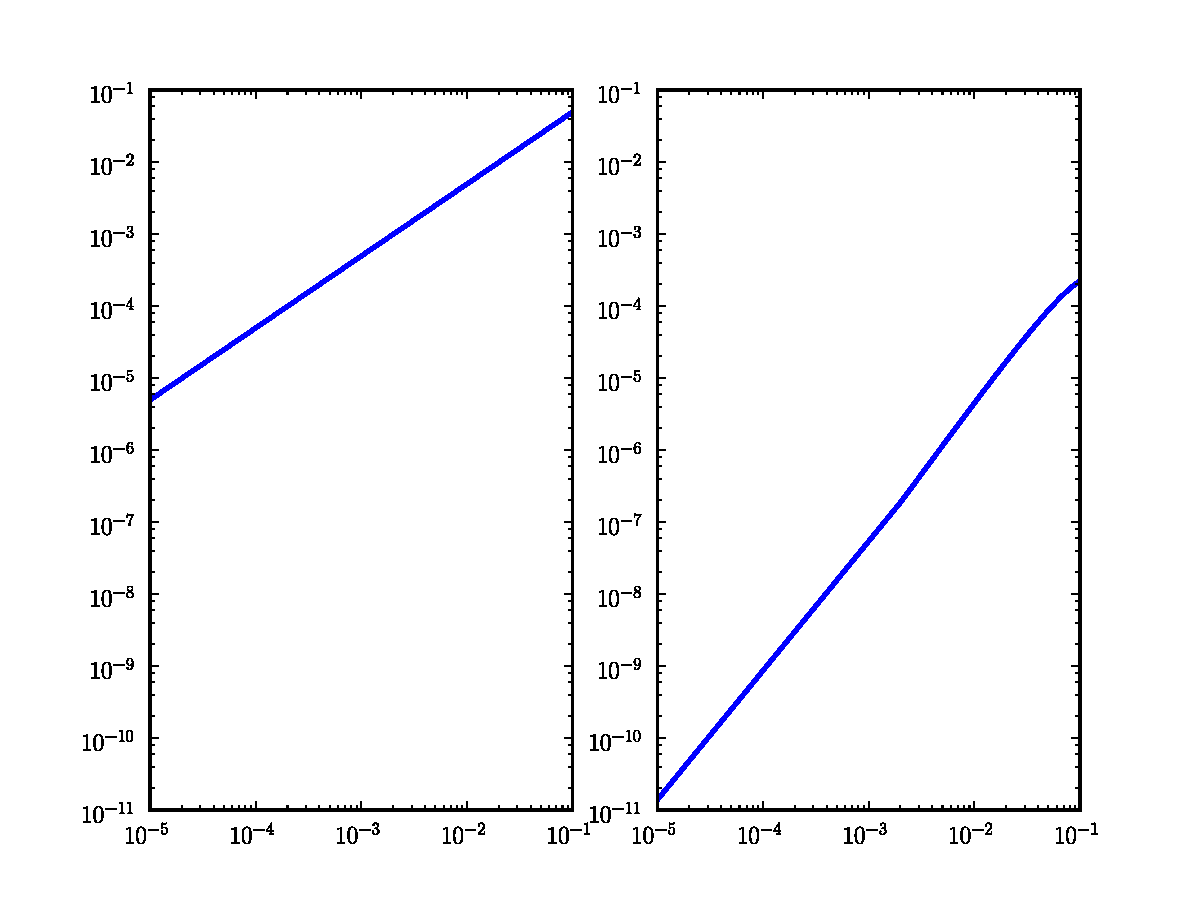
\includegraphics[width=0.8\textwidth]{convergence.pdf}
    \caption{Convergence plots for our numerical derivative approximations.
    The left plot shows the convergence for order 1 approximations. 
    The right plot shows the convergence for order 2 approximations.}
    \label{fig:convergence}
\end{figure}

\begin{problem}
Explore the convergence properties for different orders of approximation,
and for the second derivative as well. You may need to adjust your $h$
values, as they may be too small for some of the calculations.
\end{problem}
